% Options for packages loaded elsewhere
\PassOptionsToPackage{unicode}{hyperref}
\PassOptionsToPackage{hyphens}{url}
%
\documentclass[
  a4paper, xcolor = usenames,dvipsnames]{article}
\usepackage{lmodern}
\usepackage{amssymb,amsmath}
\usepackage{ifxetex,ifluatex}
\ifnum 0\ifxetex 1\fi\ifluatex 1\fi=0 % if pdftex
  \usepackage[T1]{fontenc}
  \usepackage[utf8]{inputenc}
  \usepackage{textcomp} % provide euro and other symbols
\else % if luatex or xetex
  \usepackage{unicode-math}
  \defaultfontfeatures{Scale=MatchLowercase}
  \defaultfontfeatures[\rmfamily]{Ligatures=TeX,Scale=1}
\fi
% Use upquote if available, for straight quotes in verbatim environments
\IfFileExists{upquote.sty}{\usepackage{upquote}}{}
\IfFileExists{microtype.sty}{% use microtype if available
  \usepackage[]{microtype}
  \UseMicrotypeSet[protrusion]{basicmath} % disable protrusion for tt fonts
}{}
\makeatletter
\@ifundefined{KOMAClassName}{% if non-KOMA class
  \IfFileExists{parskip.sty}{%
    \usepackage{parskip}
  }{% else
    \setlength{\parindent}{0pt}
    \setlength{\parskip}{6pt plus 2pt minus 1pt}}
}{% if KOMA class
  \KOMAoptions{parskip=half}}
\makeatother
\usepackage{xcolor}
\IfFileExists{xurl.sty}{\usepackage{xurl}}{} % add URL line breaks if available
\IfFileExists{bookmark.sty}{\usepackage{bookmark}}{\usepackage{hyperref}}
\hypersetup{
  hidelinks,
  pdfcreator={LaTeX via pandoc}}
\urlstyle{same} % disable monospaced font for URLs
\usepackage[margin=2.5cm]{geometry}
\usepackage{listings}
\newcommand{\passthrough}[1]{#1}
\lstset{defaultdialect=[5.3]Lua}
\lstset{defaultdialect=[x86masm]Assembler}
\usepackage{longtable,booktabs}
% Correct order of tables after \paragraph or \subparagraph
\usepackage{etoolbox}
\makeatletter
\patchcmd\longtable{\par}{\if@noskipsec\mbox{}\fi\par}{}{}
\makeatother
% Allow footnotes in longtable head/foot
\IfFileExists{footnotehyper.sty}{\usepackage{footnotehyper}}{\usepackage{footnote}}
\makesavenoteenv{longtable}
\usepackage{graphicx}
\makeatletter
\def\maxwidth{\ifdim\Gin@nat@width>\linewidth\linewidth\else\Gin@nat@width\fi}
\def\maxheight{\ifdim\Gin@nat@height>\textheight\textheight\else\Gin@nat@height\fi}
\makeatother
% Scale images if necessary, so that they will not overflow the page
% margins by default, and it is still possible to overwrite the defaults
% using explicit options in \includegraphics[width, height, ...]{}
\setkeys{Gin}{width=\maxwidth,height=\maxheight,keepaspectratio}
% Set default figure placement to htbp
\makeatletter
\def\fps@figure{htbp}
\makeatother
\setlength{\emergencystretch}{3em} % prevent overfull lines
\providecommand{\tightlist}{%
  \setlength{\itemsep}{0pt}\setlength{\parskip}{0pt}}
\setcounter{secnumdepth}{5}
\usepackage{setspace}
\usepackage{float}
\usepackage{fontspec}
\usepackage{subfig}
\usepackage{hyperref}
\usepackage{multirow}
\usepackage{tikz}
\usepackage[ruled]{algorithm2e}
\usepackage{siunitx}
\usetikzlibrary{chains,shapes.multipart}
\usetikzlibrary{shapes,calc,fit}
\usetikzlibrary{automata,positioning}
\floatplacement{figure}{H}
\makeatletter
\renewcommand\paragraph{\@startsection{paragraph}{4}{\z@}%
  {-2.5ex\@plus -1ex \@minus -.25ex}%
  {1.25ex \@plus .25ex}%
  {\normalfont\normalsize\bfseries}}
\makeatother
\setcounter{secnumdepth}{4}
\hypersetup{
  colorlinks = true,
}
\tikzset{
  queuei/.pic={
      \draw[line width=1pt]
      (0,0) -- ++(2cm,0) -- ++(0,-1cm) -- ++(-2cm,0);
      \foreach \Val in {1,...,3}
      \draw ([xshift=-\Val*10pt]2cm,0) -- ++(0,-1cm);
      \node[above] at (1cm,0) {$c_{#1, m_{#1}}$};
      \node[] at (0.5cm,-0.5cm) (q-#1) {};
    },
  mytri/.style={
      draw,
      shape=isosceles triangle,
      isosceles triangle apex angle=60,
      inner xsep=0.65cm
    }
}
\usepackage[style=alphabetic,backend=biber]{biblatex}
\addbibresource{ref.bib}

\author{}
\date{\vspace{-2.5em}}

\begin{document}

\onehalfspacing

\pagenumbering{gobble}

\vspace*{\fill}
\begin{center}
  \Large{\textbf{Internship report}}\\
  \vspace*{1\baselineskip}
  Vo Van Nghia\\
  \vfill
  \vspace*{\fill}
  \Large{\textbf{Date}}\\
  29 Sep, 2022
\end{center}

\newpage

\newpage
\pagenumbering{roman}
\renewcommand{\contentsname}{Table of contents}
\tableofcontents

\newpage
\pagenumbering{arabic}

\hypertarget{introduction}{%
\section{Introduction}\label{introduction}}

\hypertarget{institut-de-recherche-en-informatique-de-toulouse-irit}{%
\subsection{Institut de Recherche en Informatique de Toulouse (IRIT)}\label{institut-de-recherche-en-informatique-de-toulouse-irit}}

\hypertarget{about-the-institut}{%
\subsubsection{About the institut}\label{about-the-institut}}

The Institut de Recherche en Informatique de Toulouse (IRIT), created in 1990, is a Joint Research Unit (UMR 5505) of the Centre National de la Recherche Scientifique (CNRS), the Institut National Polytechnique de Toulouse (INP), the Université Paul Sabatier Toulouse3 (UT3), the Université Toulouse1 Capitole (UT1) and the Université de Toulouse Jean Jaurès (UT2J).

IRIT is one of the largest UMR at the national level, is one of the pillars of research in Occitanie with its 600 members, permanent and non-permanent, and about 100 external collaborators. Due to its multi-tutorial nature (CNRS, Toulouse Universities), its scientific impact and its interactions with other fields, the laboratory constitutes one of the structuring forces of the IT landscape and its applications in the digital world, both at regional and national level.

Through its cutting-edge work and dynamics, our unit has been able to define its identity and acquire undeniable visibility, while positioning itself at the heart of changes in local structures: University of Toulouse, as well as the various mechanisms resulting from future investments (LabEx CIMI, IRT Saint-Exupéry, SAT TTT, 3IA ANITI).

IRIT has focused its research on five major scientific issues and six strategic application areas.

\begin{itemize}
\tightlist
\item
  Health, Autonomy, Living, Well-being
\item
  Smart City
\item
  Aerospace and Transportation
\item
  Social Media, Digital Social Ecosystems
\item
  e-Education for learning and teaching
\item
  Heritage and People Safety
\end{itemize}

As well as strategic action:

\begin{itemize}
\tightlist
\item
  Scientific Computing, Big Data and AI
\end{itemize}

\hypertarget{organization}{%
\subsubsection{Organization}\label{organization}}

The 24 research groups of the laboratory are dispatched in seven scientific departments:

\begin{itemize}
\tightlist
\item
  Dpt ASR : Architecture, Systems, Networks
\item
  Dpt CISO : HPC, Simulation, Optimization
\item
  Dpt FSL : Reliability of Systems and Software
\item
  Dpt GD : Data Management
\item
  Dpt ICI : Interaction, Collective Intelligence
\item
  Dpt IA : Artificial Intelligence
\item
  Dpt SI : Signals, Images
\end{itemize}

\hypertarget{the-internship}{%
\subsection{The internship}\label{the-internship}}

Markov decisions processes (MDPs) and their model free counterpart in reinforcement learning (RL) have known a large success in the last two decades. Although research in these two areas has been taking place for more than fifty years, the field gained momentum only recently following the advent of powerful hardware and algorithms with which supra­human performance were obtained in games like Chess or Go. However, these impressive successes often rely on quite exceptional hardware possibilities and cannot be applied in many ''usual'' contexts, where, for instance, the volume of data available or the amount of computing power is more restricted. To define the next generation of more ''democratic'' and widely applicable algorithms, such methods still need to deal with very demanding exploration issues as soon as the state/action spaces are not small. One way around this is to use underlying knowledge and structure present in many MDPs. This is especially true for problems related to scheduling and resources sharing in among others server farms, clouds, and cellular wireless networks. The internships will revolve around this theme of improving the efficiency of learning algorithms by leveraging the structure of the underlying problem and focus mainly on model­free approach.

\hypertarget{system-settings}{%
\section{System settings}\label{system-settings}}

Two type of systems are studied in this internship: queuing system and load-balancing system.

\hypertarget{queuing-system}{%
\subsection{Queuing system}\label{queuing-system}}

\hypertarget{parameters}{%
\subsubsection{Parameters}\label{parameters}}

We have \(n\) classes of queue \(Q_{1}, \dots, Q_{n}\), and \(L_{1}, \dots, L_{n}\) the maximum number of work (limit) on each class of queue. For each \(Q_{i}\), its behavior is fully controlled by which environment it is in. An environment can be in one of the states \(m_{1}, \dots, m_{m}\). And the environment of class \(Q_{i}\) is a random variable, denoted by \(M_{i}\), which is in one of the states \(m_{1}, \dots, m_{m}\). For each environment, \(Q_{i}\) has their own holding cost \(c_{i, j}\) (the cost of one unfinished unit of work on the queue), arrival rate \(\lambda_{i, j}\) (the rate of one more unit of work arriving to the queue) and departure rate \(\mu_{i, j}\) (the rate of one unit of work on the queue has finished). Furthermore, the environment \(M_{i}\) can change from \(m_{j}\) and \(m_{k}\) with the rate of \(\xi_{i, j, k}\). In this internship, we focus on the case where \(n \coloneq 2\). A table summarizing all parameters is shown below.

\begin{table}[ht]
\caption{Queuing system parameters}
\begin{center}
\begin{tabular}{c c c c c}
    \hline
    \multicolumn{2}{c}{} & $m_{1}$ & $\dots$ & $m_{m}$ \\
    \cline{2-5}
    \multirow{3}{*}{$Q_{1}$} &  Holding cost & $c_{1, 1}$ & $\dots$ & $c_{1, m}$ \\
    & Arrival rate & $\lambda_{1, 1}$ & $\dots$ & $\lambda_{1, m}$ \\
    & Departure rate & $\mu_{1, 1}$ & $\dots$ & $\mu_{1, m}$ \\
    \cline{2-5}
    $\vdots$  \\
    \cline{2-5}
    \multirow{3}{*}{$Q_{n}$} &  Holding cost & $c_{n, 1}$ & $\dots$ & $c_{n, m}$ \\
    & Arrival rate & $\lambda_{n, 1}$ & $\dots$ & $\lambda_{n, m}$ \\
    & Departure rate & $\mu_{n, 1}$ & $\dots$ & $\mu_{n, m}$ \\
    \hline
\end{tabular}
\end{center}
\label{tab:qs-param}
\end{table}

For each \(Q_{i}\), we have a matrix transition as below.

\begin{table}[ht]
\caption{Matrix transition of the environment of $Q_{i}$}
\begin{center}
\begin{tabular}{c c c c}
    \hline
    & $m_{1}$ & $\dots$ & $m_{m}$ \\
    $m_{1}$ & $\xi_{i, 1, 1}$ & \dots & $\xi_{i, 1, m}$ \\
    \vdots \\
    $m_{m}$ & $\xi_{i, m, 1}$ & \dots & $\xi_{i, m, m}$ \\
    \hline
\end{tabular}
\end{center}
\label{tab:mat-transition-ci}
\end{table}

The state of the system is represented by two vectors:

\begin{itemize}
\tightlist
\item
  \(S = (X_{1}, \dots, X_{n})\) where \(X_{i}\) is a random variable represents the current number of works of class \(Q_{i}\) and is observable.
\item
  \(E = (M_{1}, \dots, M_{n})\) and this vector is not observable.
\end{itemize}

\hypertarget{cost}{%
\subsubsection{Cost}\label{cost}}

The cost of the system is a function of \(S\) and \(E\). We propose two functions of cost. The first one is a simple linear function.

\[
f_{1}(S, E) = \sum_{1}^{n} c_{i, M_{i}} X_{i}
\]

And the second one is a convex function which is specialized for the case \(n = 2\), where \(\epsilon\) is a fixed positive constant.

\[
f_{2}(S, E) = c_{1, M_{1}} X_{1} + c_{2, M_{2}} (\epsilon X_{2}^{2} + X_{2})
\]

\hypertarget{agent}{%
\subsubsection{Agent}\label{agent}}

The agent will decide which queues should be activated. His goal is to minimize the cost of the whole system. Only works on activating queues can be processed and finished. In more generic problems, the agent is allowed to activate / deactivate multiple queues at the same time based on some conditions. However, in this internship, the agent can only activate one queue at a time.

\begin{figure}
\centering
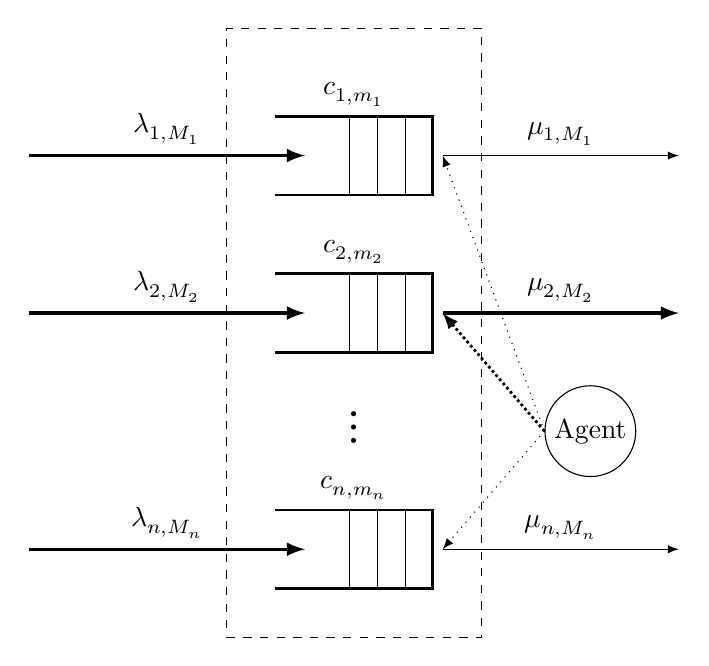
\begin{tikzpicture}[>=latex]
% the shapes
\path
  (0,3cm) pic {queuei=1}
  (0,1cm) pic {queuei=2}
  (0,-2cm) pic {queuei=n};
\path
  (1,4cm) coordinate (aux1)
  (1,-3.5cm) coordinate (aux2)
  (-0.5,0cm) coordinate (aux3)
  (2.5,0cm) coordinate (aux4);
\node[draw,dashed,text width=2.5cm,fit={(aux1) (aux2) (aux3) (aux4)}] (dashed) {};
\node[draw,align=center,circle,inner sep=2pt]
  at (4,-1) (agent)
  {Agent};

%the arrows
\draw[->, line width=1.25]
  ([xshift=-3.5cm]q-1.west) --
    node[anchor=south,align=center] {$\lambda_{1, M_{1}}$}
  (q-1.west);
\draw[->]
  ([xshift=1.5cm]q-1.east) --
    node[anchor=south,align=center] {$\mu_{1, M_{1}}$}
  ([xshift=4.5cm]q-1.east);
\draw[->, line width=1.25]
  ([xshift=-3.5cm]q-2.west) --
    node[anchor=south,align=center] {$\lambda_{2, M_{2}}$}
  (q-2.west);
\draw[->, line width=1.25]
  ([xshift=1.5cm]q-2.east) --
    node[anchor=south,align=center] {$\mu_{2, M_{2}}$}
  ([xshift=4.5cm]q-2.east);
\draw[->, line width=1.25]
  ([xshift=-3.5cm]q-n.west) --
    node[anchor=south,align=center] {$\lambda_{n, M_{n}}$}
  (q-n.west);
\draw[->]
  ([xshift=1.5cm]q-n.east) --
    node[anchor=south,align=center] {$\mu_{n, M_{n}}$}
  ([xshift=4.5cm]q-n.east);
\draw[->,dotted]
  (agent.west) --
    node[anchor=south,align=center] {}
  ([xshift=1.5cm]q-1.east);
\draw[->,densely dotted, line width=1]
  (agent.west) --
    node[anchor=south,align=center] {}
  ([xshift=1.5cm]q-2.east);
\draw[->,dotted]
  (agent.west) --
    node[anchor=south,align=center] {}
  ([xshift=1.5cm]q-n.east);
\path ([xshift=0.5cm]q-2.south) -- ([xshift=0.5cm]q-n.north) node [font=\LARGE, midway, sloped] {$\dots$};
\end{tikzpicture}
\caption[Visualization of the queueing system when the agent activates queue 2]{Visualization of the queueing system when the agent activates queue 2, the bold lines represent the flow of works inside the system.}
\end{figure}

\hypertarget{evolution}{%
\subsubsection{Evolution}\label{evolution}}

In the continuos-time scale, each type of event (work arrival, work departure and environment changing) happens independently. That system is quite hard to program, therefore, we used a technique called ``uniformization'' to move from the continuos-time scale to discrete-time scale. In this time scale, at a given time, only one event can take place, regardless of their type.

In particular, given the system state is \((S, E)\), the agent decides to activate queue \(a\). One of these \(n + 1 + n(m - 1) + 1\) events can happen.

\begin{itemize}
\tightlist
\item
  The work of class \(Q_{i}\) increases by 1. Because there are \(n\) classes, we have \(n\) events of this kind with the rate \(\lambda_{1, M_{1}}, \dots, \lambda_{n, M_{n}}\) respectively (if the number of work of class \(Q_{i}\) reaches an upper limit, we consider \(\lambda_{i, M_{i}} = 0\)).
\item
  The work of class \(Q_{a}\) decreases by 1. Because we can only activate only one class, there is only one event of this type and its rate is \(\mu_{a, M_{a}}\).
\item
  The environment of class \(Q_{i}\) changes to a different environment other than \(m_{i}\) and the rate changing to environment \(j\) is \(\xi_{i, M_{i}, j}\). Because there are \(m - 1\) possible changes for each class and there are \(n\) classes, the number of this kind of event is \(n(m - 1)\).
\item
  And a special dummy event where nothing changes.
\end{itemize}

A discrete probability distribution is used to express that. In order to satisfy the condition of a probability distribution, all the rates above are divided by a normalization constant \(C\) to make sure that their sum are not greater than 1. If that sum is smaller than 1, the special dummy event is used to fill the gap so that the final sum will be equal to 1.

The normalization constant has the form as follow, which is deduced from the above evolution of the system.

\[
C = \sum_{i = 1}^{n} \max_{j} \lambda_{i, j} + \max_{i, j} \mu_{i, j} + \sum_{i = 1}^{n} \max_{j} \sum_{k = 1, k \neq j}^{m} \xi_{i, j, k} + \epsilon
\]

If \(\epsilon > 0\), the probability of the dummy event will always be greater than 0. In this internship, as we do not want the system evolves too slowly, we choose \(\epsilon \coloneq 0\).

After obtaining all the information above, we use that discrete probability distribution to obtain the next transition \(T\) of the system and denote \(S'\) and \(E'\) the next state of the system.

\hypertarget{load-balancing-system}{%
\subsection{Load-balancing system}\label{load-balancing-system}}

\hypertarget{parameters-1}{%
\subsubsection{Parameters}\label{parameters-1}}

For this system, we have a similar parameters with the one of the queuing system. The only difference in this system is that instead of having multiple arrival rate that depends on the class of queue as well as the environment, we have only one global arrival rate \(\lambda\). A table summarizing the parameters of this system is shown below.

\begin{table}[ht]
\caption{Load-balancing system parameters}
\begin{center}
\begin{tabular}{c c c c c}
    \hline
    \multicolumn{2}{c}{} & $m_{1}$ & $\dots$ & $m_{m}$ \\
    \cline{2-5}
    \multirow{2}{*}{$Q_{1}$} &  Holding cost & $c_{1, 1}$ & $\dots$ & $c_{1, m}$ \\
    & Departure rate & $\mu_{1, 1}$ & $\dots$ & $\mu_{1, m}$ \\
    \cline{2-5}
    $\vdots$  \\
    \cline{2-5}
    \multirow{2}{*}{$Q_{n}$} &  Holding cost & $c_{n, 1}$ & $\dots$ & $c_{n, m}$ \\
    & Departure rate & $\mu_{n, 1}$ & $\dots$ & $\mu_{n, m}$ \\
    \cline{2-5}
    & Global arrival rate & & $\lambda$ & \\
    \hline
\end{tabular}
\end{center}
\label{tab:lbs-param}
\end{table}

\hypertarget{cost-1}{%
\subsubsection{Cost}\label{cost-1}}

Same as above, the cost of the system is a function of \(S\) and \(E\). However, in this system, only the simple linear version is used.

\[
f_{1}(S, E) = \sum_{1}^{n} c_{i, M_{i}} X_{i}
\]

\hypertarget{agent-1}{%
\subsubsection{Agent}\label{agent-1}}

The goal of the agent is the same: minimizing the cost of the whole system. The difference here is instead of having to deactivating some queues, all queues now run continuously. His mission is to choose which queue to send the new arriving work to. Only the chosen queue will have new work arriving, the other queues only have to process the remaining works of them.

\begin{figure}
\centering
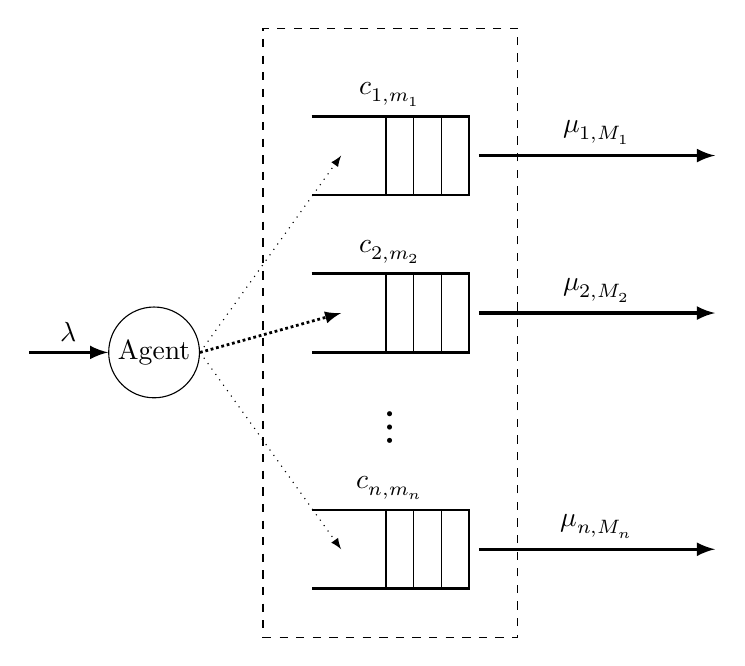
\begin{tikzpicture}[>=latex]
% the shapes
\path
  (0,3cm) pic {queuei=1}
  (0,1cm) pic {queuei=2}
  (0,-2cm) pic {queuei=n};
\path
  (1,4cm) coordinate (aux1)
  (1,-3.5cm) coordinate (aux2)
  (-0.5,0cm) coordinate (aux3)
  (2.5,0cm) coordinate (aux4);
\node[draw,dashed,text width=2.5cm,fit={(aux1) (aux2) (aux3) (aux4)}] (dashed) {};
\node[draw,align=center,circle,inner sep=2pt]
  at (-2,0) (agent)
  {Agent};

%the arrows
\draw[->, line width=1.25]
  ([xshift=-1cm]agent.west) --
    node[anchor=south,align=center] {$\lambda$}
  (agent.west);
\draw[->, dotted]
  (agent.east) --
    node[anchor=south,align=center] {}
  (q-1.west);
\draw[->, line width=1.25]
  ([xshift=1.5cm]q-1.east) --
    node[anchor=south,align=center] {$\mu_{1, M_{1}}$}
  ([xshift=4.5cm]q-1.east);
\draw[->, densely dotted, line width=1]
  (agent.east) --
    node[anchor=south,align=center] {}
  (q-2.west);
\draw[->, line width=1.25]
  ([xshift=1.5cm]q-2.east) --
    node[anchor=south,align=center] {$\mu_{2, M_{2}}$}
  ([xshift=4.5cm]q-2.east);
\draw[->, dotted]
  (agent.east) --
    node[anchor=south,align=center] {}
  (q-n.west);
\draw[->, line width=1.25]
  ([xshift=1.5cm]q-n.east) --
    node[anchor=south,align=center] {$\mu_{n, M_{n}}$}
  ([xshift=4.5cm]q-n.east);
\path ([xshift=0.5cm]q-2.south) -- ([xshift=0.5cm]q-n.north) node [font=\LARGE, midway, sloped] {$\dots$};
\end{tikzpicture}
\caption[Visualization of the load-balancing system when the agent sends work to queue 2]{Visualization of the load-balancing system when the agent sends work to queue 2, the bold lines represent the flow of works inside the system.}
\end{figure}

\hypertarget{evolution-1}{%
\subsubsection{Evolution}\label{evolution-1}}

In this system, given its state is \((S, E)\), the agent decides to send work to queue \(a\). One of these \(1 + n + n(m - 1) + 1\) events can happen.

\begin{itemize}
\tightlist
\item
  The work of class \(Q_{a}\) increases by 1. Because we can only send work to one queue, there is only one event of this type and its rate is \(\lambda\).
\item
  The work of class \(Q_{i}\) decreases by 1. Because there are \(n\) classes, we have \(n\) events of this kind with the rate \(\mu_{1, M_{1}}, \dots, \mu_{n, M_{n}}\) respectively (if the number of work of class \(Q_{i}\) reaches 0, we consider \(\mu_{i, M_{i}} = 0\)).
\item
  The environment of class \(Q_{i}\) changes to a different environment other than \(m_{i}\) and the rate changing to environment \(j\) is \(\xi_{i, M_{i}, j}\). Because there are \(m - 1\) possible changes for each class and there are \(n\) classes, the number of this kind of event is \(n(m - 1)\).
\item
  And a special dummy event where nothing changes.
\end{itemize}

The form of the normalization constant also changes according to the evolution of the system.

\[
C = \lambda + \sum_{i = 1}^{n} \max_{j} \mu_{i, j} + \sum_{i = 1}^{n} \max_{j} \sum_{k = 1, k \neq j}^{m} \xi_{i, j, k} + \epsilon
\]

\hypertarget{system-representation}{%
\subsection{System representation}\label{system-representation}}

In this internship, we limited ourselves on the cases where \(n = 2\) for both systems. A system of that kind can be represented as a grid whose each side represents the evolution of each queue. In this report, we use the vertical side for the first queue, and the horizontal one for the second. Each cell of that grid represent a specific observable state of the system.

\begin{figure}
\centering
\def\mycolumns{5}
\def\myrows{5}
\begin{tikzpicture}[x=1cm, y=1cm, mynums/.style={inner sep=0}]
\fill[gray!50] (1,1) -- +(0, 1) -- +(1, 1) -- +(1,0) -- cycle;
\draw[step=1cm] (0,0) grid (\mycolumns + 1,\myrows + 1);
\foreach\x in {0,...,\mycolumns}
  \node[anchor=south, mynums] at (\x+0.5, \myrows + 1.25) {\x};
\foreach\x in {0,...,\myrows}
  \node[anchor=east, mynums] at (-0.25, \myrows - \x + 0.5) {\x};
\draw[->]
  (-1, \myrows + 0.5) --
    node[anchor=east,align=center] {$Q_{1}$}
  (-1, 0.5);
\draw[->]
  (0.5, \myrows + 2) --
    node[anchor=south,align=center] {$Q_{2}$}
  (\mycolumns + 0.5, \myrows + 2);
\end{tikzpicture}
\caption[Representation of a system with 2 queues]{Representation of a system with 2 queues and the length limit of both queues are 5, the gray cell represents an observable state of the system $S = (4, 1)$}
\end{figure}

\hypertarget{reinforcement-learning}{%
\section{Reinforcement learning}\label{reinforcement-learning}}

Reinforcement learning is used for training the agent to attain his goal. In this session, we present a short summary and introduce some related notions that could be useful for later.

\hypertarget{parameters-2}{%
\subsection{Parameters}\label{parameters-2}}

A simple reinforcement learning is modeled by a markov decision process (MDP) whose parameters include as follow:

\begin{itemize}
\tightlist
\item
  \(\mathcal{S}\): the set of all states of the system.
\item
  \(\mathcal{A}\): the set of all actions, and \(A_{S}\), the set of all actions available from state \(S\).
\item
  \(P(S_{t + 1} = S' | S_{t} = S, a_{t} = a)\): the probability that action \(a\) in state \(S\) at time \(t\) will lead to state \(S'\) at time \(t + 1\).
\item
  \(R(S' | S, a)\): the immediate reward received after transitioning from state \(S\) to state \(S'\), due to action \(a\).
\end{itemize}

In addition, we have policy \(\pi(a | S) = \mathbb{P}[A_{t} = a | S_{t} = S]\), a distribution over actions given states. In our problem, there is also an unobservable state inside our system, therefore, our problem is a generalization of the MDP, called partial observable markov decision process (POMDP). The parameters could be seen as follow:

\begin{itemize}
\tightlist
\item
  \(\mathcal{S}\): the set of observable states is represented as the grid.
\item
  \(\mathcal{E}\): the set of unobservable environment states.
\item
  \(\mathcal{A}\): the action of activating / sending work to a queue.
\item
  \(P(S', E' | S, E, a)\): the transition probability that is clarified in the evolution section and depends on the both visible and hidden state (S, E).
\item
  \(R(S' | S, E, a)\): the immediate reward is \(-C\) where \(C\) is the total holding cost of the system. Since this function depends only on the the state (S, E) of system, we could write \(R(S, E)\) instead.
\end{itemize}

\hypertarget{bellman-equation}{%
\subsection{Bellman equation}\label{bellman-equation}}

First, we want to try the solving method of a MDP to our problem, so in this section, we assume that \(E\) is a constant state and will not consider \(E\).

The accumulate discounted future reward (return) from time \(t\) with the discount factor \(0 \le \gamma \le 1\) is:
\[
G_{t} = r_{t + 1} + \gamma r_{t + 2} + \gamma^{2} r_{t + 3} + \gamma^{3} r_{t + 4} + \dots = r_{t + 1} + \gamma G_{t + 1}
\]

From that, we have state-value function \(V_{\pi}(S)\) is the expected return starting from state \(S\), and then following policy \(\pi\):

\begin{equation}
V_{\pi}(S) = \mathbb{E}_{\pi}[G_{t} | S_{t} = S]
\label{eq:state-value}
\end{equation}

And action-value function \(Q_{\pi}(S, a)\) is the expected return starting from state \(S\), taking action \(a\), and then following policy \(\pi\):

\begin{equation}
Q_{\pi}(S, a) = \mathbb{E}_{\pi}[G_{t} | S_{t} = S, a_{t} = a]
\label{eq:action-value}
\end{equation}

From the fact that \(\pi(a | S)\) is a distribution over \(\mathcal{A}\) given \(S\), we have:

\begin{equation}
\begin{split}
V_{\pi}(S) {}&= \mathbb{E}_{\pi}[G_{t} | S_{t} = S] \\
  &= \sum_{a \in \mathcal{A}} \pi(a | S) \mathbb{E}_{\pi}[G_{t} | S_{t} = S, a_{t} = a] \\
  &= \sum_{a \in \mathcal{A}} \pi(a | S) Q_{\pi}(S, a)
\label{eq:v-to-q}
\end{split}
\end{equation}

Furthermore, we see that the expected future return of \(Q_{\pi}(S, a)\) is the sum of the current reward \(R(S)\) as well as the expected return of the next state regardless action multiply by the probability of moving to that state. Therefore, we have the equation below:

\begin{equation}
Q_{\pi}(S, a) = R(S) + \gamma \sum_{S' \in \mathcal{S}} P(S' | S, a) V_{\pi}(S')
\label{eq:q-to-v}
\end{equation}

Finally, the bellman equations are obtained from \eqref{eq:v-to-q} and \eqref{eq:q-to-v}:

\begin{align}
\begin{split}
V_{\pi}(S) {}&= \sum_{a \in \mathcal{A}} \pi(a | S) Q_{\pi}(S, a) \\
  &= \sum_{a \in \mathcal{A}} \pi(a | S) (R(S) + \gamma \sum_{S' \in \mathcal{S}} P(S' | S, a) V_{\pi}(S')) \\
  &= R(S) + \gamma \sum_{a \in \mathcal{A}} \pi(a | S) \sum_{S' \in \mathcal{S}} P(S' | S, a) V_{\pi}(S')
\label{eq:bellman-v-1}
\end{split} \\
\begin{split}
Q_{\pi}(S, a) {}&= R(S) + \gamma \sum_{S' \in \mathcal{S}} P(S' | S, a) V_{\pi}(S') \\
  &= R(S) + \gamma \sum_{S' \in \mathcal{S}} P(S' | S, a) \sum_{a' \in \mathcal{A}} \pi(a' | S') Q_{\pi}(S', a')
\label{eq:bellman-q-1}
\end{split}
\end{align}

\hypertarget{optimal-policy}{%
\subsection{Optimal policy}\label{optimal-policy}}

The core idea of this problem is to find an optimal policy \(\pi_{*}\) that maximizes the expected reward or \(V(S)\). Mathematically, we have
\[
\pi > \pi' \text{ if } V_{\pi}(S) > V_{\pi'}(S) \,\, \forall S \in \mathcal{S}
\]

And we want to find
\[
\pi_{*} \text{ such that } \pi_{*} \ge \pi \,\, \forall \pi
\]

We can do that by finding the optimal state-value function \(V_{*}(S) = \max_{\pi} V_{\pi}(S)\) or action-value function \(Q_{*}(S, a) = \max_{\pi} Q_{\pi}(S, a)\) and define the optimal policy as follow:
\[
\pi_{*}(S) = \begin{cases}
1 & \text{ if } a = \arg\max_{a \in \mathcal{A}} Q_{*}(S, a) \\
0 & otherwise
\end{cases}
\]

Plug all together into equation \eqref{eq:bellman-v-1} and \eqref{eq:bellman-q-1}, we have:

\begin{align}
V_{*}(S) &= R(S) + \max_{a \in \mathcal{A}} \gamma \sum_{S' \in \mathcal{S}} P(S' | S, a) V_{*}(S')
\label{eq:bellman-max-v} \\
Q_{*}(S, a) &= R(S) + \gamma \sum_{S' \in \mathcal{S}} P(S' | S, a) \max_{a' \in \mathcal{A}} Q_{*}(S', a')
\label{eq:bellman-max-q}
\end{align}

We then move to next sections where we discuss about several training methods based on these equations.

\hypertarget{online-q-learning}{%
\section{Online Q-learning}\label{online-q-learning}}

\hypertarget{about-the-algorithm}{%
\subsection{About the algorithm}\label{about-the-algorithm}}

Online Q-learning is probably one of the most simple and popular algorithm for reinforcement learning problem. It is used to estimate \(Q_{*}(S, a) \,\, \forall S \in \mathcal{S} \text{ and } a \in \mathcal{A}\) while interacting with the system. This algorithm only requires the real system or a simulator to interact with, and not the internal settings of that system, which makes it fit the context of this internship and more broadly real-life, where these settings can change at any time. Beside its simplicity and close to real life context, the algorithm is also proven to converge almost surely when the number of visit to each state goes to \(\infty\) in \autocite{q-learning-converge}. Visually, we can imagine that our agent will follow a grid trajectory of states and try to discover what is the action-value at that state with a specific action.

\begin{figure}
\centering
\def\mycolumns{5}
\def\myrows{5}
\begin{tikzpicture}[x=1cm, y=1cm, mynums/.style={inner sep=0}]
\fill[gray!50] (0,5) -- +(0, 1) -- +(1, 1) -- +(1,0) -- cycle;
\draw[step=1cm] (0,0) grid (\mycolumns + 1,\myrows + 1);
\foreach\x in {0,...,\mycolumns}
  \node[anchor=south, mynums] at (\x+0.5, \myrows + 1.25) {\x};
\foreach\x in {0,...,\myrows}
  \node[anchor=east, mynums] at (-0.25, \myrows - \x + 0.5) {\x};
\draw[->]
  (-1, \myrows + 0.5) --
    node[anchor=east,align=center] {$Q_{1}$}
  (-1, 0.5);
\draw[->]
  (0.5, \myrows + 2) --
    node[anchor=south,align=center] {$Q_{2}$}
  (\mycolumns + 0.5, \myrows + 2);
\draw[->, line width=1.25] (0.5, 5.5) -- (1.5, 5.5) -- (1.5, 3.5) -- (0.5, 3.5) -- (0.5, 2.5) -- (3.5, 2.5);
\end{tikzpicture}
\caption[An example of the path which the agent might take]{An example of the path which the agent might take. It starts from $(0, 0)$ and moves to $(3, 3)$. The next state could be either $(3, 4), (4, 3), (3, 2), (2, 3)$ depends on the action it chooses and the transition probabilities.}
\end{figure}

Formally, the algorithm can be written as follow:

\begin{algorithm}
\caption{Online Q-Learning}\label{alg:on-q-learning}
\KwIn{$T > 0$ number iterations, $\gamma$ discount factor, $\epsilon$ exploration factor, $\eta$ learning rate}
\KwOut{$Q_{*}$, $\pi_{*}$}
\tcc{Internally, $\mathfrak{S}$ keeps track of the unobservable state $E$ as well but the algorithm can not extract it here.}
$\mathfrak{S}$ simulator of the system\;
\For {$t \gets 0$ \KwTo $T$} {
  $S \gets \mathfrak{S}$ current observable state of the system\;
  $a \gets 
    \begin{cases}
    \begin{aligned}
      \text{one random possible action}&, && \text{ with the probability of } \epsilon \text{ (exploration)}\\ 
      \arg\max_{a \in \mathcal{A}} Q_{t}(S, a)&, && \text{ with the probability of } 1 - \epsilon \text{ (learning)}
    \end{aligned}
    \end{cases}
  $\\
  \tcc{The state $E$ might change in this step but from the algorithm's perspective, nothing has changed.}
  $R, S' \gets \mathfrak{S}(a)$\;
  $Q_{t+1}(S, a) \gets Q_{t}(S, a) + \eta (R + \gamma \max_{a' \in \mathcal{A}} Q_{t}(S', a'))$ \;
}
\end{algorithm}

\hypertarget{implementation}{%
\subsection{Implementation}\label{implementation}}

\hypertarget{from-python-to-c}{%
\subsubsection{From Python to C++}\label{from-python-to-c}}

In this section, we document the some difficulties while implementing the framework and how we overcome it. For illustration purpose, we will test the algorithm with a very simple problem of the \protect\hyperlink{queuing-system}{queuing system}
and linear cost function with no environment (or constant environment). The parameter of this system is show in table \ref{tab:q-learning-test}.

\begin{table}[ht]
\caption{Simple queuing problem for testing}
\begin{center}
\begin{tabular}{c c c}
    \hline
    \multirow{3}{*}{$Q_{1}$} & Holding cost $c_{1}$ & $2$ \\
    & Arrival rate $\lambda_{1}$ & $0.135$ \\
    & Departure rate $\mu_{1}$ & $0.3$ \\
    \cline{2-3}
    \multirow{3}{*}{$Q_{2}$} & Holding cost $c_{2}$ & $3$ \\
    & Arrival rate $\lambda_{2}$ & $0.135$ \\
    & Departure rate $\mu_{2}$ & $0.3$ \\    
    \hline
\end{tabular}
\end{center}
\label{tab:q-learning-test}
\end{table}

It has been proven that if we have \(c_{1} \mu_{1} \ge c_{2} \mu_{2}\), the optimal policy for all cases is activating the first queue if possible, and vice versa in the case where \(c_{1} \mu_{1} \le c_{2} \mu_{2}\). From table \ref{tab:q-learning-test}, we know that our optimal action here is activating the second queue.

With a naive Python implementation, the algorithm works correctly when the limit of both queue are small.

\begin{figure}

{\centering \includegraphics[width=0.4\linewidth]{report_files/figure-latex/3x3-python-1} 

}

\caption{Result of online Q-learning using Python for 3x3 case. $\gamma = 0.999$, $\epsilon = 0.99$}\label{fig:3x3-python}
\end{figure}

First, we see that on the first column where \(Q_{2} = 0\), our agent always chooses to activate the first queue, not because this is the optimal action but this is the only option possible, because there is no work on the second queue. Same thing holds for the first row where \(Q_{1} = 0\). For the other cells, we have the black color which means the agent chooses the second queue which is aligned with the analytical solution as above.

This implementation runs \(10^6\) iterations for approximately \(2\) minutes. This is quite good for number with small case. However, if we increase the limit to 10, with the same number of iterations gives a imperfect result.

\begin{figure}

{\centering \subfloat[For $10^6$ iterations\label{fig:10x10-python-1}]{\includegraphics[width=0.4\linewidth]{report_files/figure-latex/10x10-python-1} }\subfloat[For $10^7$ iterations\label{fig:10x10-python-2}]{\includegraphics[width=0.4\linewidth]{report_files/figure-latex/10x10-python-2} }

}

\caption{Result of online Q-learning using Python for 10x10 case. $\gamma = 0.99$, $\epsilon = 0.999$}\label{fig:10x10-python}
\end{figure}

In the figure above, we can see that even after 20 minutes with \(10^7\) iterations, the algorithm still does not converge completely yet. To have a clear view about the reason ưhy, we have figure \ref{fig:10x10-python-n-visit}.

\begin{figure}

{\centering \subfloat[Activating $Q_{1}$\label{fig:10x10-python-n-visit-1}]{\includegraphics[width=0.4\linewidth]{report_files/figure-latex/10x10-python-n-visit-1} }\subfloat[Activating $Q_{2}$\label{fig:10x10-python-n-visit-2}]{\includegraphics[width=0.4\linewidth]{report_files/figure-latex/10x10-python-n-visit-2} }

}

\caption{Number of visit for the system above. $\gamma = 0.99$, $\epsilon = 0.999$}\label{fig:10x10-python-n-visit}
\end{figure}

We can see that, our agent is stuck at \((0, 0)\), only the area around the origin has a high number of visit. The rest have relatively low visit and therefore, does not converge because of the nonfulfillment of the condition in \autocite{q-learning-converge}.

To speed up the algorithm, we decided to switch to C++, which is famous for its speed and its mature support for high-speed computation with library like \passthrough{\lstinline!Eigen!} and then expose a Python interface for more ease of use. This is also the same approach for many scientific libraries in Python such as \passthrough{\lstinline!Numpy!} or \passthrough{\lstinline!Tensorflow!}. After switching to C++ and some improvements later, the algorithm now can run \(10^9\) iterations in only 1 minutes, a \(2 \times 10^3\) speed up.

\hypertarget{from-n-dimensions-to-2-dimensions}{%
\subsubsection{\texorpdfstring{From \(n\)-dimensions to \(2\)-dimensions}{From n-dimensions to 2-dimensions}}\label{from-n-dimensions-to-2-dimensions}}

With C++, the simulator is already running faster. However, there are still room for improvements. Now, the probability \(P(S', E' | S, E, a)\) is calculated on-the-fly when we meet that state \((S, E)\) while running the algorithm, we could make it faster by calculate the matrix transition for all the states beforehand. However, the state \(S\) and \(E\) of the system are each represented by a vector of \(n\) entries, if we keep using vector like that, we will need a tensor of \(n + n + 1 = 2N + 1\) dimensions (first \(n\) dimensions for saving the observable state \(S\), the next \(n\) dimensions for saving the unobservable state \(S\) and the last one for action). In addition, since there is no sparse version for high-dimensional tensor, it will take a lot of memories to save that tensor, more precisely:

\[
(L_{1} + 1) \times \dots \times (L_{n} + 1) \times \underbrace{n^{m}}_{n \text{ queues and } m \text{ environments}} \times \underbrace{n}_{n \text{ actions}}
\]

If we try to allocate a tensor of that size, we will get an ``out of memory'' error.

Furthermore, in other algorithms, we are required to iterate all over the set of states. If \(n\), the number of queues is static, we could something similar to algorithm \ref{alg:states-3}. However our goal is to let \(n\) as a input for the program. So we can not use that algorithm there.

\begin{algorithm}
\caption{Iteration over the set of visible states $\mathcal{S}$ when $n = 3$} \label{alg:states-3}
\For {$i \gets 0$ \KwTo $L_{1}$} {
  \For {$j \gets 0$ \KwTo $L_{2}$} {
    \For {$k \gets 0$ \KwTo $L_{3}$} {
      $S \gets (i, j, k)$\;
      \dots\;
    }
  }
}
\end{algorithm}

In the end, we decide to encode the whole state into an integer by extending the notion of base of number. Given state \((S, E)\), we introduce 3 functions:
\[
\begin{aligned}
f_{\mathcal{S}}(S) &= f(X_{1}, \dots, X_{n}) = X_{1} L_{2} \dots L_{n} + X_{2} L_{3} \dots L_{n} + \dots + X_{n - 1} L_{n} + X_{n} \\
f_{\mathcal{E}}(E) &= f(M_{1}, \dots, M_{n}) = M_{1} m^{n - 1} + M_{2} m^{n - 2} + \dots + M_{n - 1} m + M_{n} \\
f_{\mathcal{S, E}(S, E)} &= f(X_{1}, \dots, X_{n}, M_{1}, \dots, M_{n}) = m^{n} f_{\mathcal{S}}(S) + f_{\mathcal{E}}(E)
\end{aligned}
\]

All three functions are one-to-one mapping, so we can replace the state with the result of these function without losing anything. Because of doing so, we have achieved several benefits:

\begin{itemize}
\tightlist
\item
  We can calculate the transition matrix right now and use a sparse matrix to store it for efficiency in both storage and performance (since the transition matrix will be full of 0).
\item
  Turn a problem with unknown dimension to a 2-dimensional one which makes accessing and looping through the states easier.
\item
  Overall speed improvement since we only need to deal with integer instead of a vector.
\end{itemize}

\hypertarget{result}{%
\subsection{Result}\label{result}}

\hypertarget{offline-q-learning}{%
\section{Offline Q-learning}\label{offline-q-learning}}

\hypertarget{about-the-algorithm-1}{%
\subsection{About the algorithm}\label{about-the-algorithm-1}}

In this version of Q-learning, we do not explore or follow the trajectory as in the online version, but we will force calculate the q value for all pair \((S, a)\). This method is faster than online Q-learning, however, it requires a reliable simulator of the system to be able to work. The algorithm could be described below:

\begin{algorithm}
\caption{Offline Q-Learning}\label{alg:off-q-learning}
\KwIn{$T > 0$ number iterations, $\gamma$ discount factor, $\eta$ learning rate}
\KwOut{$Q_{*}$, $\pi_{*}$}
$\mathfrak{S}$ simulator of the system\;
$E$ initial environment state of the system\;
\For {$t \gets 0$ \KwTo $T$} {
  $ -, -, E' \gets \mathfrak{S}(-, -, E)$\;
  \If{$E \ne E'$}{
    $E \gets E'$ \;
  }
  \For {$S \in \mathcal{S}$} {
    \For {$a \in \mathcal{A}$} {
      $S', R, - \gets \mathfrak{S}(a, S, E)$\;
      $Q_{t+1}(S, a) \gets Q_{t}(S, a) + \eta (R + \gamma \max_{a'} Q_{t}(S', a'))$\;
    }
  }
}
\end{algorithm}

\hypertarget{result-1}{%
\subsection{Result}\label{result-1}}

\hypertarget{value-iteration}{%
\section{Value iteration}\label{value-iteration}}

\hypertarget{about-the-algorithm-2}{%
\subsection{About the algorithm}\label{about-the-algorithm-2}}

This algorithm is directly based on equation \eqref{eq:bellman-max-v} and used to estimate the value of \(V_{*}(S)\). After obtaining an estimate of \(V_{*}(S)\), the policy is deduced as \(\pi_{*}(S) = \arg\max_{a} R(S) + \gamma \sum_{S' \in \mathcal{S}} P(S' | S, a) V_{*}(S')\). The algorithm is written as follow:

\begin{algorithm}
\caption{Value iteration} \label{alg:value-iteration}
\KwIn{$\gamma$ discount factor}
\KwOut{$V_{*}$, $\pi_{*}$}
$\Delta \gets \infty$\;
\While {\Delta > \epsilon} {
  \For {$S \in \mathcal{S}$} {
    $V_{t+1}(S) \gets \max_{a \in \mathcal{A}} R(S) + \gamma \sum_{S' \in \mathcal{S}} P(S' | S, a) V_{*}(S')$\;
  }
  $\Delta \gets \lVert V_{t + 1} - V_{t} \rVert$\_{2};
}
\end{algorithm}

We can see above that the algorithm makes use of \(P(S' | S, a)\), because of this, this algorithm converge a lot faster than both Q-learning methods but it does not fit into the goal of the internship since we have to know the transition probability, so this method is use only as a baseline to compare with the result of Q-learning. Furthermore, if we have only one constant environment \(E_{c}\) (or no environment changing), we could rewrite \(P(S', E_{c} | S, E_{c}, a) = P(S' | S, a)\) and value iterations work correctly. However, adding environment will eventually break the algorithm because we have \(P(S', E' | S, E, a)\) but we want to estimate \(V_{*}(S)\) and not \(V_{*}(S, E)\). In the next section, we discuss about how to get an empirical estimate of \(P(S'|S, a)\) based on \(P(S', E' | S, E, a)\).

\hypertarget{empirical-transition-probability}{%
\subsection{Empirical transition probability}\label{empirical-transition-probability}}

Our idea is to calculate the probability of the system stay in a particular state \(E \in \mathcal{E}\) and then multiply it with the transition probability to get the average probability. First, we have some equations:

\begin{equation}
  P(S'|S, E, a) = 
    \begin{cases}
        P(S', E|S, E, a) \quad & \text{if} \, S' \neq S \\
        1 - \sum_{S' \neq S} P(S', E|S, E, a) = \sum_{E'} P(S, E'|S, E, a) \quad & \text{otherwise} \\
    \end{cases}
\label{eq:p-s}
\end{equation}

\begin{equation}
  P(E'|S, E, a) = 
    \begin{cases}
        P(S, E'|S, E, a) \quad & \text{if} \, E' \neq E \\
        1 - \sum_{E' \neq E} P(S, E'|S, E, a) \quad & \text{otherwise} \\
    \end{cases}
\label{eq:p-e}
\end{equation}

The logic behind equation \eqref{eq:p-s} and \eqref{eq:p-e} is the fact that there is only one event can happen at a time.

\begin{equation}
  P(S, E'|S, E, a) = 
    \begin{cases}
        \xi_{i, M_{i}, M_{i}'} \quad & \text{if} \, E' \text{ and } E \text{ differ by only one entry at index } i \\
        0 \quad & \text{else} \\
    \end{cases}
\label{eq:p-e-e}
\end{equation}

By rewriting \(P(S, E' | S, E, a)\) as in equation \eqref{eq:p-e-e}, we see that \(P(E'|S, E, a)\) does not depend on \(S, a\) and therefore \(P(E'|S, E, a) = P(E'| E)\). From that, we could calculate the steady state by an iterative method using the equation below:

\begin{equation}
\label{eqn:steady_prob}
    \pi_{t + 1}(E') = \sum_{E \in \mathcal{E}} P(E'| E) \pi_{t}(E)
\end{equation}

After \(\pi(E)\) converges to \(\tilde{\pi}(E)\) and using \eqref{eq:p-s}, we have the final empirical value we want:

\begin{equation}
\label{eqn:p_tilde}
    \tilde{P}(S'| S, a) = \sum_{E \in \mathcal{E}} \tilde{\pi}(E) P(S'| S, E, a)
\end{equation}

\hypertarget{result-2}{%
\subsection{Result}\label{result-2}}

\hypertarget{comparison}{%
\section{Comparison}\label{comparison}}

\newpage

\printbibliography

\end{document}
